% !TEX root = ../main.tex
\chapter{Introduction}\label{ch:chapter1} % For referencing the chapter elsewhere, use \ref{Chapter1}

%----------------------------------------------------------------------------------------
Video is the medium to record, copy, playback, broadcast
and display the motion images in an electronic style~\parencite{RN190}.
Watching videos is becoming an important way for our entertainment as well
as education.
The high definition (HD) and ultra high definition (UHD) video
are increasingly demanding nowadays.
People prefer videos with higher definitions than those with lower
resolutions because the former one provides much better viewing experience.
However, challenges emerged for delivering videos with high definition.
HD videos typically contain much more information in every picture frame than the
standard definition videos.
More data needs to be squeezed into the same capacity for transmission.
For example, the uncompressed video with the dimension \(720\times480\) at 30 frames
per second requires 0.03 gigabytes per second, while the uncompressed video with
the dimension \(2880\times2048\) at 120 frames per second requires 2.12 gigabytes per
second.
Since bit rate is proportional to system bandwidth for
transmission~\parencite{RN191}, and expanding the bandwidth in a large scale is
too expensive, the significantly increased bit rate
for transmitting the video data is becoming one of the
major obstacles for HD video services.

To cope with the growing need for higher compression of moving
pictures~\parencite{RN193}, Joint Collaborative Team on Video
Coding (JCT-VC)~\parencite{RN192} has developed the High Efficiency Video
Coding standard which is the newest international video coding standard for
substantially ameliorate the compression performance against the previous
standards.
Comparing with the H.264 Advanced Video Compression Standard~\parencite{RN194},
the H.265 High Efficiency Video Coding Standard provides fifty percent bit rate
reduction while maintaining the objective video quality at the same level.

While Two-dimensional video is the most common video type,
Three-dimensional (3D) video has been brought to market via lots of ways,
including Blu-Ray disc, cable and satellite transmission, terrestrial
broadcast, and streaming or downloading from the Internet~\parencite{RN118}.
3D video provides the perception of depth information which augments
the vividness of the video contents.
Currently most 3D videos in the market are using stereo display technology.
Two similar views, one for left eye, the other for right eye, are presented
at the same time with the multiplexing techniques enabling the
adjustments of video geometry information~\parencite{RN196} to provide
the 3D effect.
Figure~\ref{fig:stereo-display} illustrates the typical system structure for
transmitting videos targeting stereo display.
\begin{figure}
    \centering
    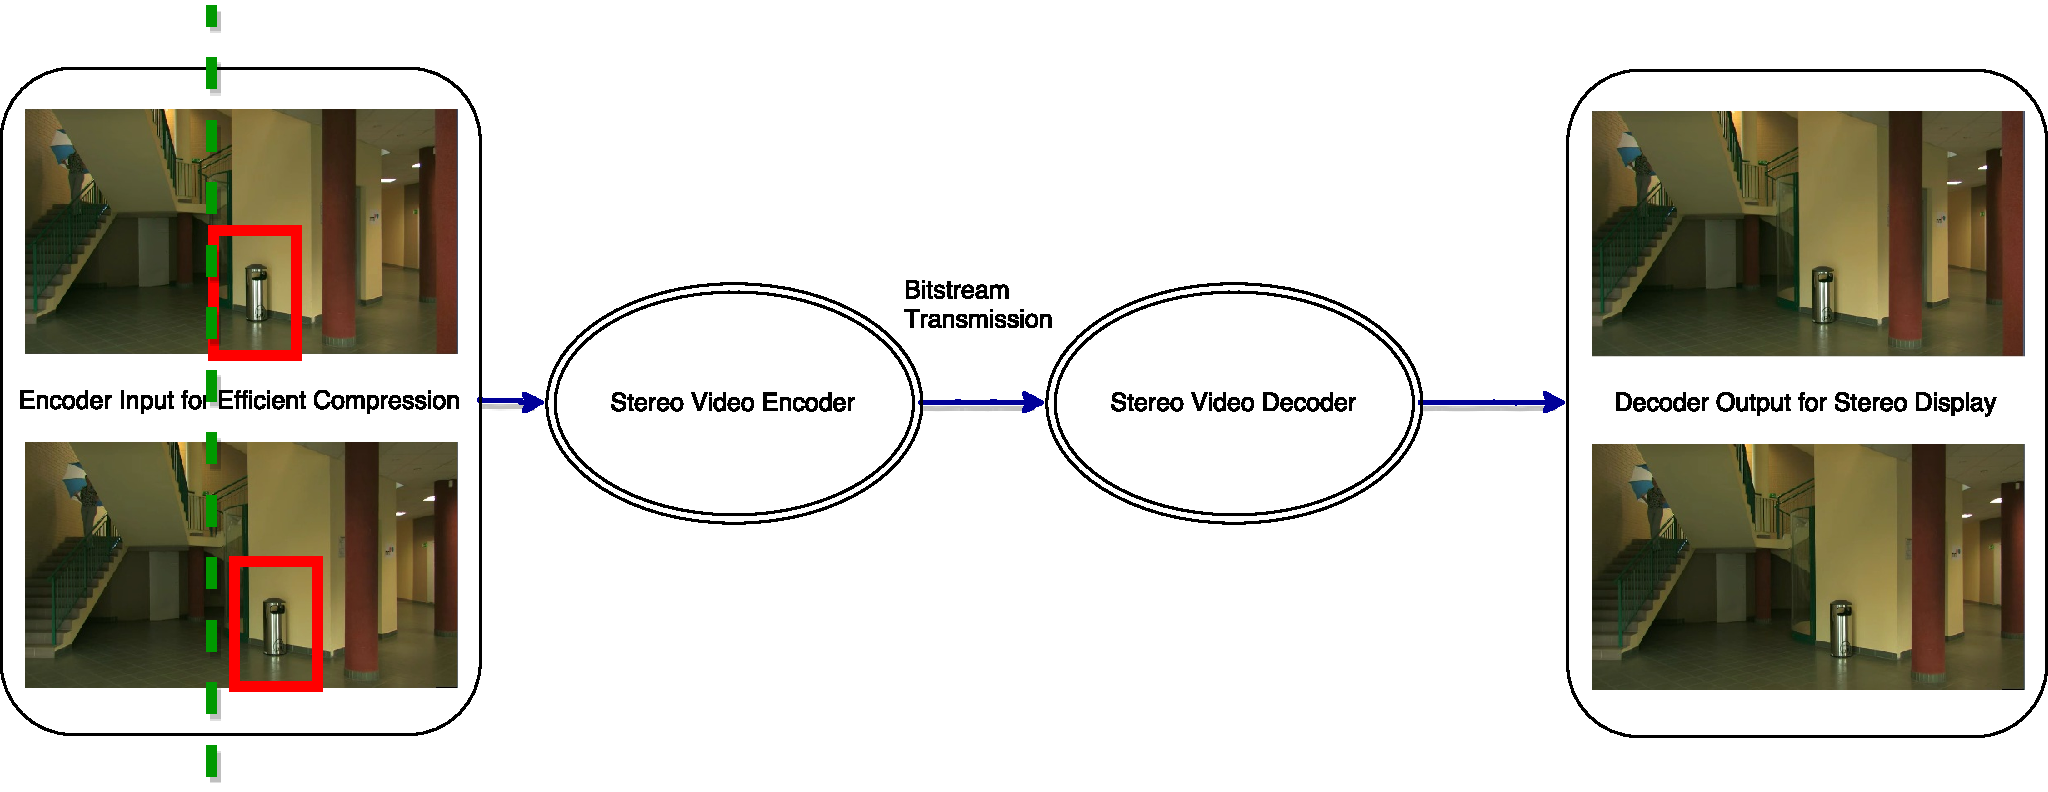
\includegraphics[
        width=\textwidth,
        height=\textheight,
        keepaspectratio
        ]{Figures/StereoDisplay.pdf}
    \caption[System Structure for transmitting videos targeting 
    stereo display]{System Structure for transmitting videos
     targeting stereo display.}\label{fig:stereo-display}
\end{figure}
It can be observed that there exists a displacement between the
two views.
The green vertical left margins of the red rectangles in the two views
at encoder side are different.
Such a displacement is the visual disparity for 3D perception.
Stereoscopic videos~\parencite{RN153} have
achieved great profitability for movie theatres in recent years.
For example, IMAX 3D has became the most popular one that offering
the immersing multimedia experiences around the world.
Special 3D glasses are needed for watching the IMAX 3D movies.
The current 3D film industry is very successful in terms of attracting
customers, however, it is not the end of the story.
Myopic people do not like to wear one more pair of glasses when
watching 3D movies.
Some people will experience discomfort after wearing the 3D glasses for a
period of two hours.
To get rid of the undesired 3D glasses,
autostereoscopic multi-view technology~\parencite{RN153} is coming to
our rescue.
The two major different characteristics between stereo display and
autostereoscopic display are
listed in Table~\ref{tab:diff-stereo-autostereo}~\parencite{RN44}.
\begin{table}[b]
    \caption{Characteristics comparison of stereoscopic display and autostereoscopic display}
    \bigskip\label{tab:diff-stereo-autostereo}
    \centering
    \begin{tabular}{c c c}
        \toprule
        Characteristic & Stereo Display & Autostereoscopic Display\\
        \midrule
        Glass-Free & No & Yes \\
        Multiple Stereo Pairs & No & Yes \\
%        Number of Views & two views & more than two views \\
%        Overall Display Resolution & High & Low \\
%        Perceivable Scene Depth Quality & High & Low \\
        \bottomrule
    \end{tabular}
\end{table}
The impact of different view numbers for autostereoscopic display is shown in
Table~\ref{tab:autostereo-less-views-more-views}~\parencite{RN44}.
\begin{table}
    \caption{Impact of Available View Amount for Autostereoscopic Display}
    \bigskip\label{tab:autostereo-less-views-more-views}
    \centering
    \begin{tabular}{c c c}
        \toprule
        Characteristic & Small Number of Views & Large Number of Views \\
        \midrule
        Seamless View Transition  & No & Yes \\
        High Quality of Scene Depth & No & Yes \\
        \bottomrule
    \end{tabular}
\end{table}
Comparative ease can be brought to the 3D video audience
since they do not need to wear 3D glasses for watching autostereoscopic videos.
At each different view position, scenes with minor differences are available
from multiple stereo pairs which are provided by autostereoscopic
display~\parencite{RN44}.
As a result, when audience make a move for various view positions, scenes
not viewable from the previous locations are revealed during the movement.
The autostereoscopic multi-view display demands more than two views.
With a sufficient amount of views present in autostereoscopic display, the
disparities between every two adjacent views can be small enough to offer
seamless transitions from scene to scene, such that when multiple views
meet eyes sequentially, the scenes as a whole can be gorgeous.
The visual quality of the autostereoscopic display is highly proportional to
the number of available views.
Due to limited available bandwidth, transmitting arbitrary number of views
is not practical.
Researchers have proposed a new format which only requires limited number
of view and their associated depth maps for the capability of
generating arbitrary amount of views theoretically.
The typical system structure for using this new format to compress and supply 3D video
resources is shown in Figure~\ref{fig:SS-MVD}.
An enormous amount of views in the medium positions which are able to
guarantee the high quality of the 3D video can be synthesized from
\begin{figure*}[!b]
    \centering
    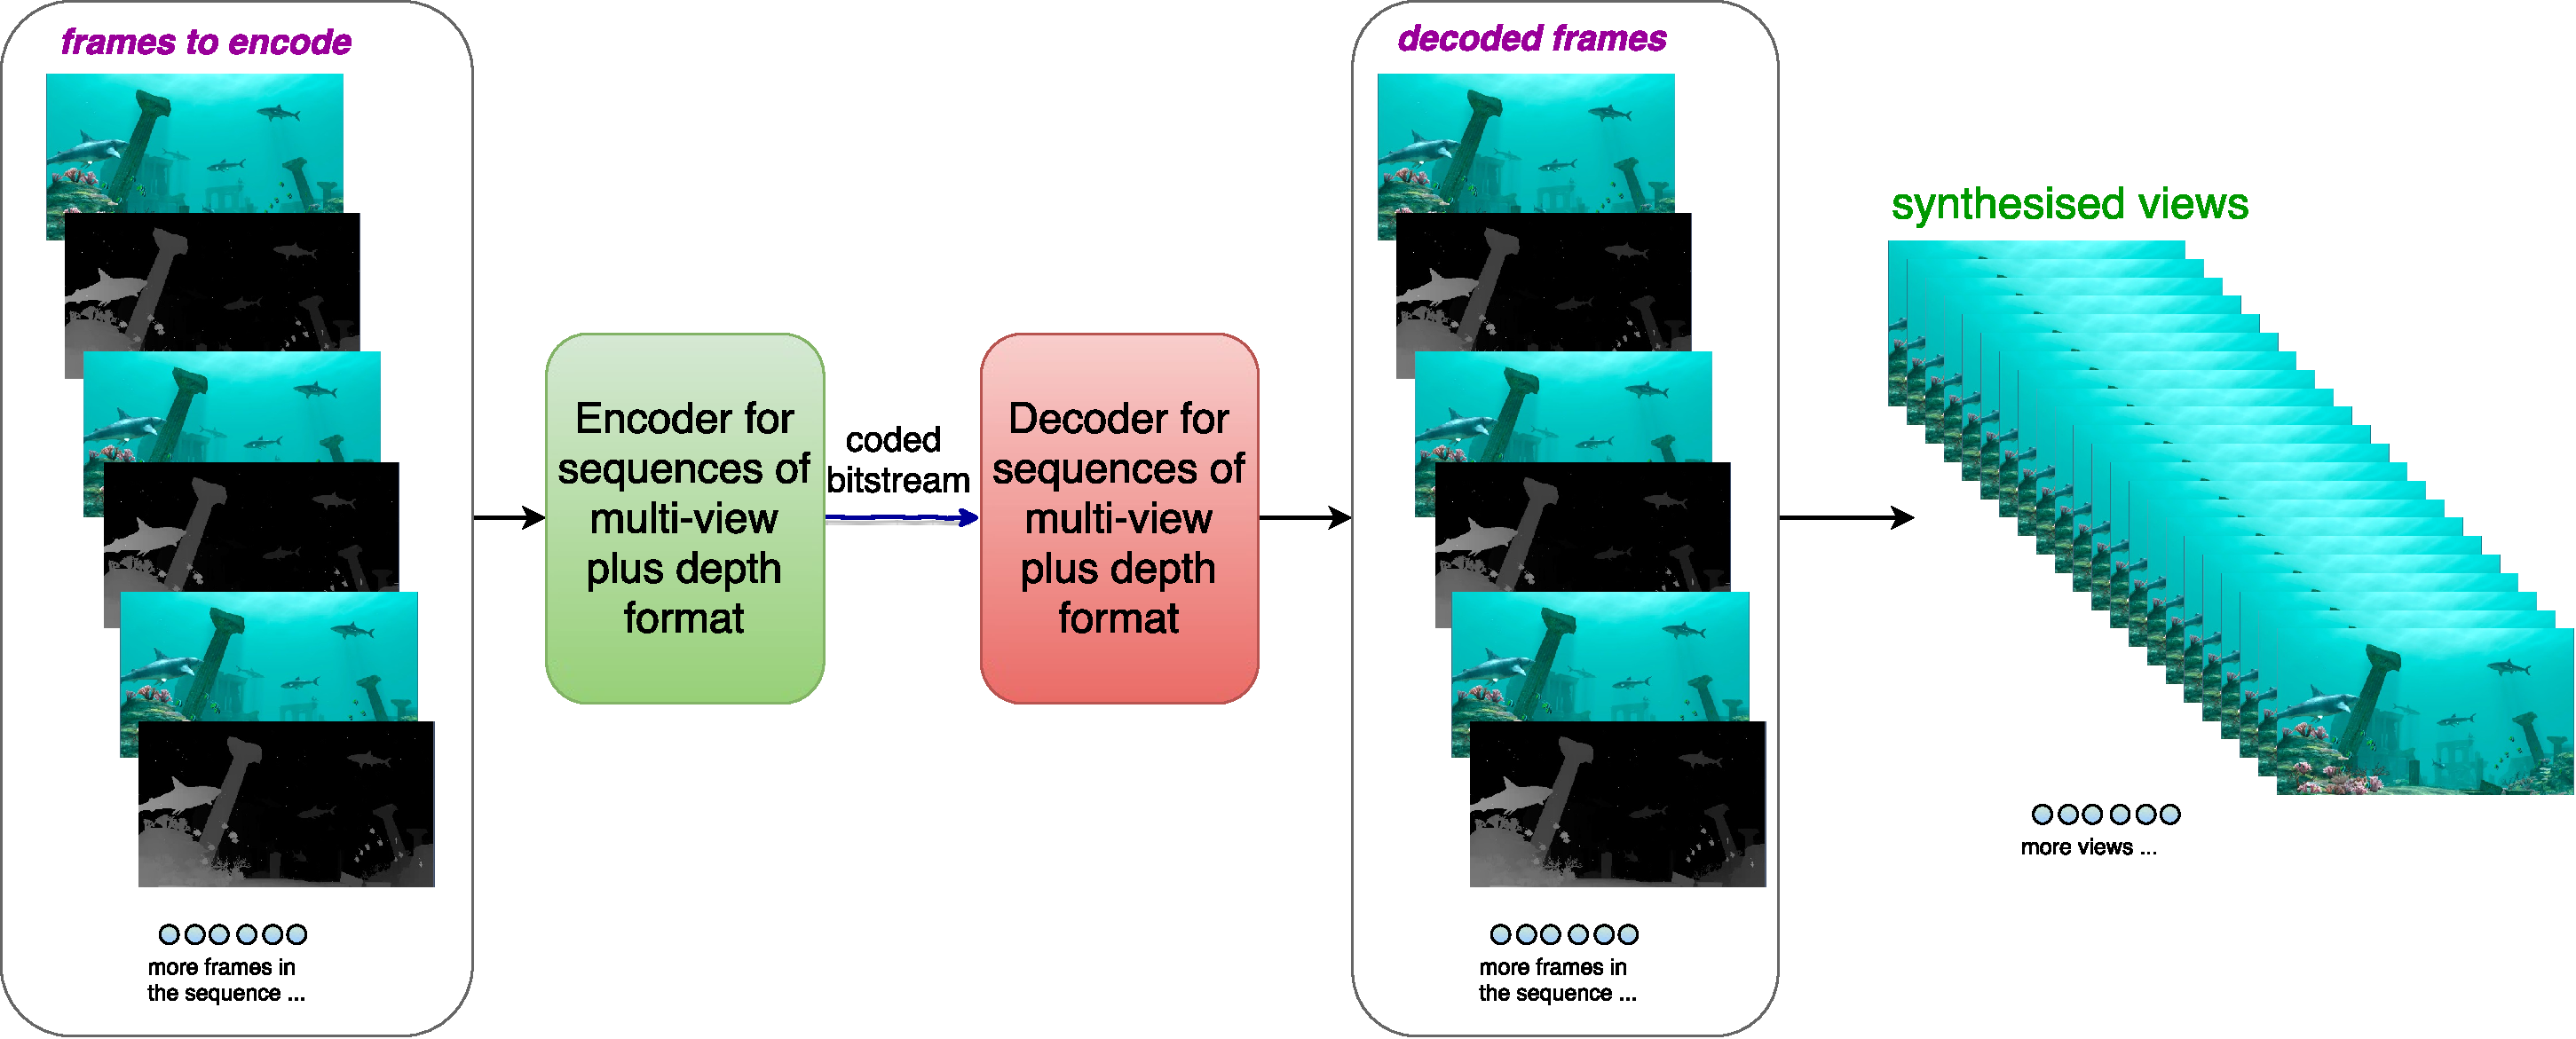
\includegraphics[width=\textwidth,height=\textheight,keepaspectratio]{Figures/SystemStructureOf3DEncoder}
%        \decoRule
    \caption[System Structure for transmitting videos of Multi-view 
    Plus Depth format]{System Structure for transmitting videos of 
    Multi-view Plus Depth format.}\label{fig:SS-MVD}
\end{figure*}
the decoded texture frames in combination with decoded depth maps.
%The multi-view plus depth format provides the functionality of synthesizing
%required number of views from texture views and associated depth maps.\\

To employ multi-view plus depth format for 3D video, efficient compressing
methods are desired, which has led to the 3D Video Coding Extension of the
High Efficiency Video Coding Standard (3D-HEVC) by the Joint Collaborative Team
on 3D Video Coding Extension Development (JCT-3V)~\parencite{RN195}.
The 3D Extension of the HEVC standard gives extra coding efficiency
for encoding a few texture views along with the corresponding depth maps by
using new tools which exploit the redundancies amongst
texture and depth views, and pay attention to the unique characteristics of
the depth maps, such as large homogeneous
regions separated by sharp boundaries~\parencite{RN47}.

Depth information measures of the distance between the object in the far position
and the object in the near position from a static viewpoint,
which is expressed in the format of depth map.
\begin{figure*}[!t]
    \centering
    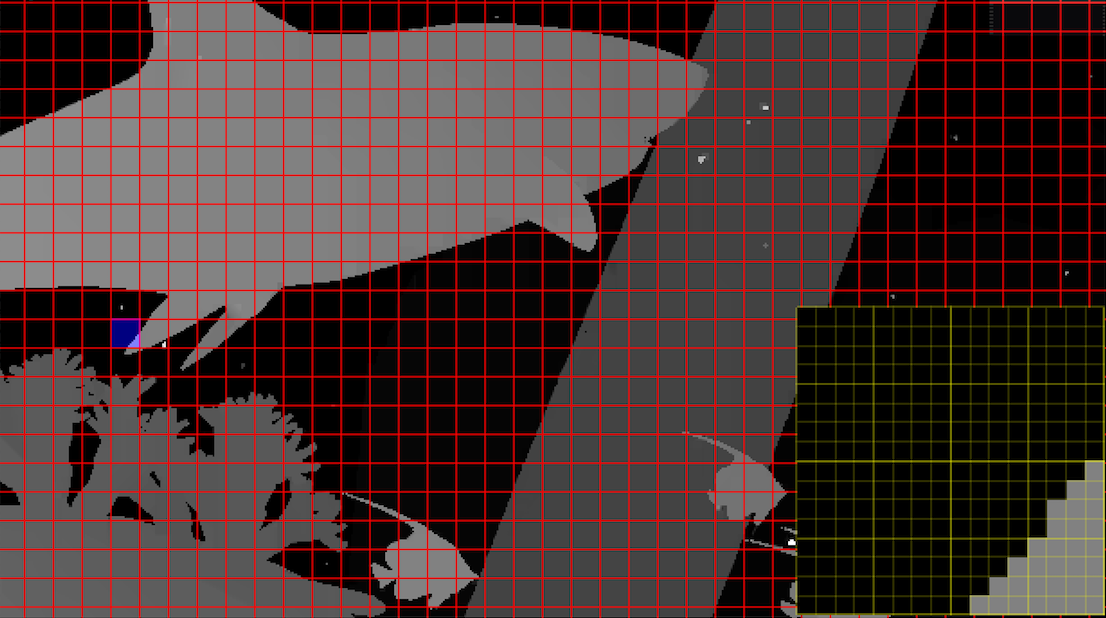
\includegraphics[width=\textwidth,height=\textheight,keepaspectratio]{Figures/wedgelet}
%        \decoRule
    \caption[Wedgelet partition illustration]
    {Example of wedgelet partition in a block of size 
    16 by 16 in depth map
    from Shark video sequence.
    }\label{fig:wedgelet-partition}
\end{figure*}
Instead of presenting depth maps directly to the viewer, views in the medium
positions are generated by Depth-Image-Based Rendering (DIBR) technique.
The qualities of the depth maps are vital to the DIBR process.
Corona artifacts (a.k.a.\ ringing artifacts)~\parencite{RN44}
can be discovered in synthesized
views if the edge sharpness in depth maps can not be well
preserved.
Therefore, retaining the edge sharpness in depth map is the key to avoid the
artifacts in the synthesized views.
In 3D-HEVC, new intra-picture prediction tools and residual coding methods
have been applied to preserve the special properties of depth maps.
Depth Modelling Mode (DMM) which is one of the new intra-picture
prediction tools, is designed to provide much more granularity for
encoding the depth maps than the normal angular intra prediction modes.
DMM is more capable of approximating the depth maps to be encoded due to
the fact that it provides a vast amount of non-rectangle partitions.
Figure~\ref{fig:wedgelet-partition} presents an example of the wedgelet
partition from the depth map in Shark video sequence.
The small block highlighted by blue color amongst the blocks
separated by the red grid is magnified at the right-bottom position in
Figure~\ref{fig:wedgelet-partition}.
A straight line is used for the partition in wedgelet mode.
Figure~\ref{fig:contour-partition} shows a sample of the contour partition
from the same depth map as Figure~\ref{fig:wedgelet-partition}.
The partition pattern comprises contour lines instead of one single
straight line.
Wedgelet partition and contour partition for depth maps
are enabled by DMM1 and DMM4 separately.
%The wedgelet partition is shown in Figure.
%The contour partition is shown in Figure.
%~\parencite{RN197}.
\begin{figure}
    \centering
    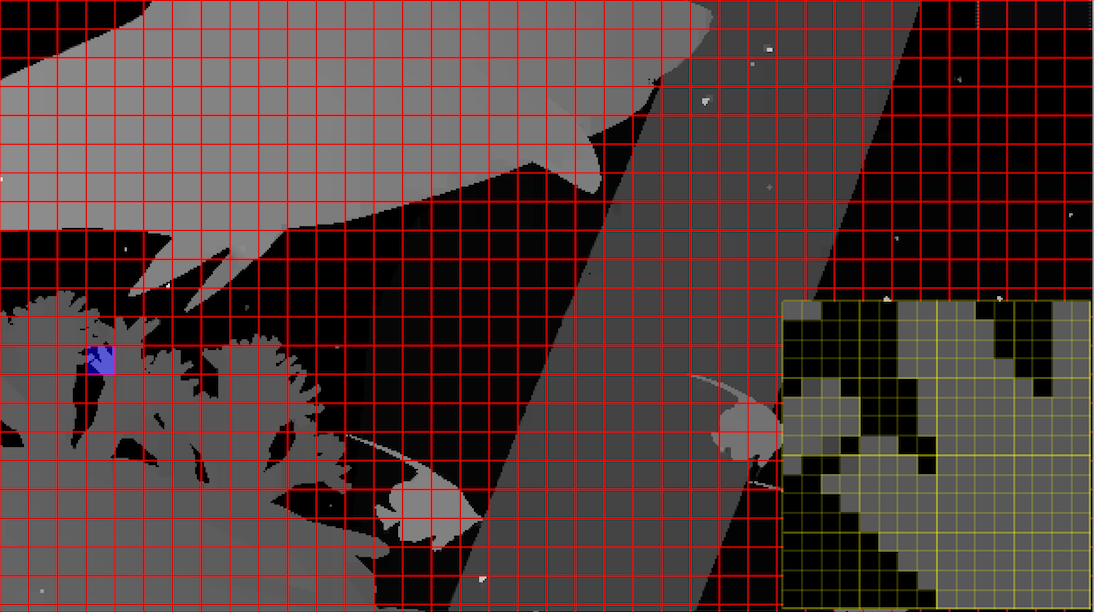
\includegraphics[width=\textwidth,height=\textheight,keepaspectratio]{Figures/contour}
%        \decoRule
    \caption[Contour partition illustration]
    {Example of contour partition in a block of size 16 by 16 in depth map
    from Shark video sequence.
    }\label{fig:contour-partition}
\end{figure}
%introduce a little about depth map and their usage.
%mentioning iphonex true depth camera.
%draw the picture

%----------------------------------------------------------------------------------------

\section{Motivation}\label{sec:motivation_and_contribution}
The idea of this work originates from the discovery of the computational
complexity of the wedgelet searching process in depth modelling modes.
The immense complexity for searching the best wedgelet candidate lead to
the strongly marked increase of encoding time.
The time consumed for compressing a single depth map in 3D-HEVC encoder is
roughly a sixfold increase relevant to the encoding time of a single texture
frame wherein the all intra configuration in HTM-16.2 is used.
Thus we designed a deep neural network architecture which is trained
subsequently for predicting the most probable wedgelet candidates.
The learned model achieves 92.2\% to 97.3\% top-16 accuracy for various
block sizes.
The inference engine is integrated into the reference software
(HTM-16.2) of 3D-HEVC\@.
The learned models reduce roughly half of the wedgelet searching candidates.
It provides 64.6\% time reduction in average while the BD performance
has a negligible decrease comparing with the unmodified 3D-HEVC encoder.

\textbf{Motivation for Wedgelet Candidates Reduction:} The encoding time
consumed in HTM-16.2 encoder for
each view (including both texture and depth) by default can be
observed from the command line outputs.
Figure~\ref{fig:encoding-time-example} shows a piece of command line outputs
from the encoding process of Shark sequence.
\begin{figure}
    \centering
    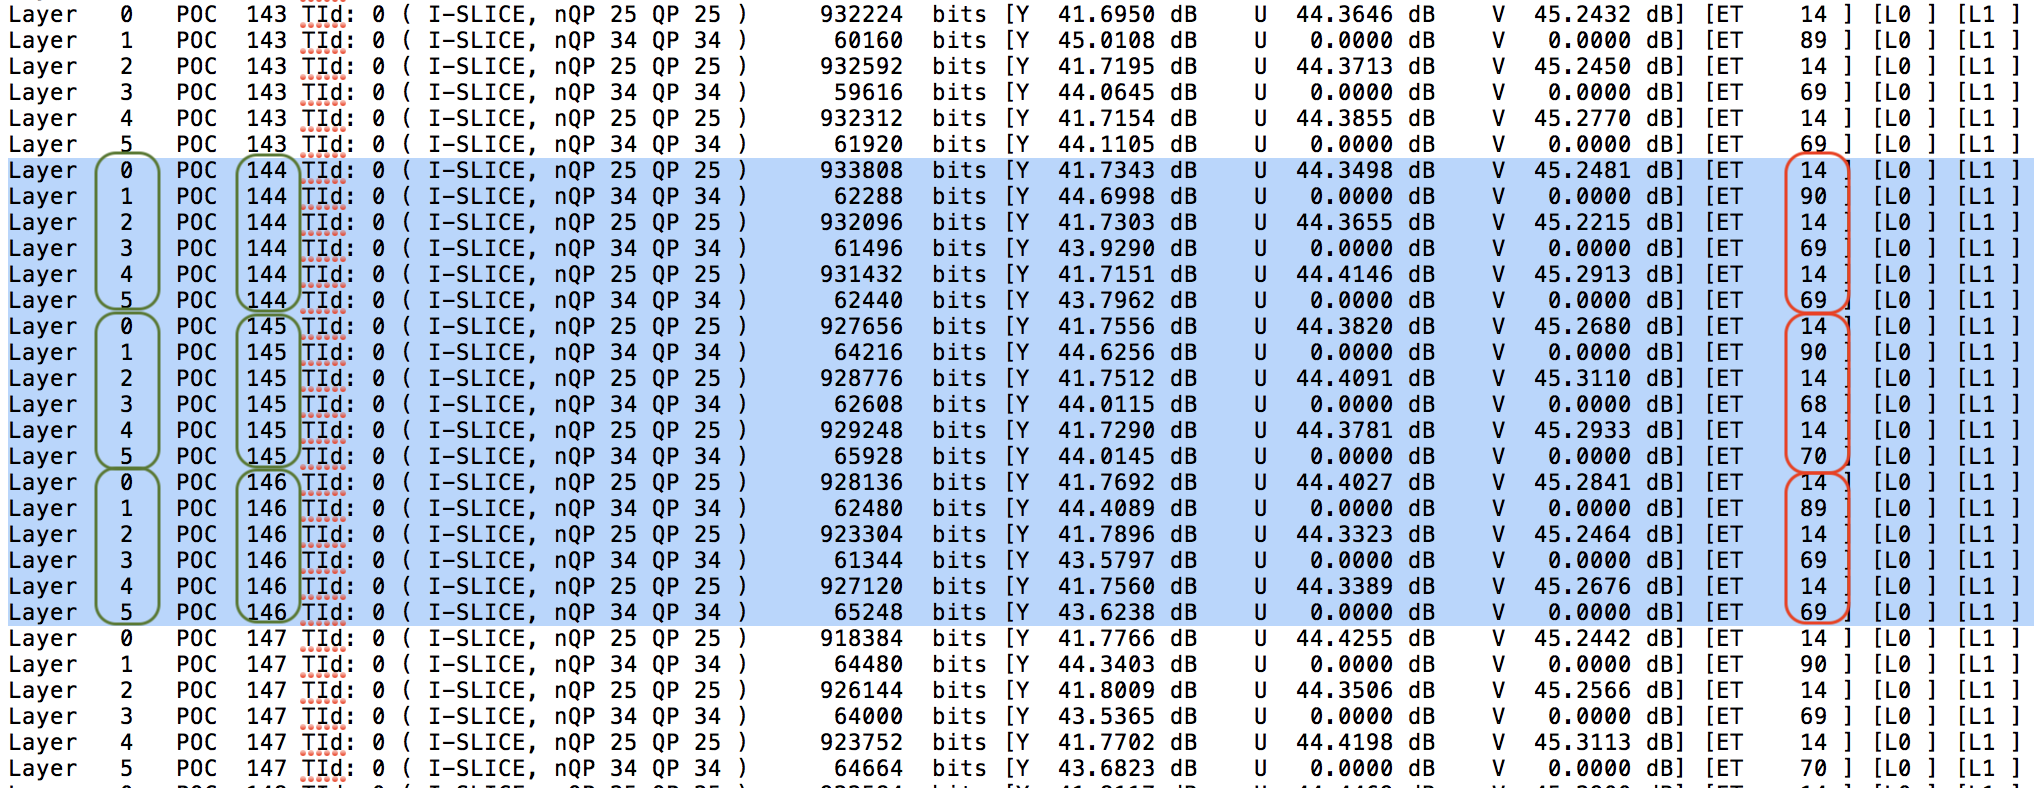
\includegraphics[width=\textwidth,height=\textheight,keepaspectratio]{Figures/EncodingTimeEg}
%        \decoRule
    \caption[An example showing a piece of the command line outputs during
    the encoding process for Shark sequence]
    {An example showing a piece of the command line outputs during the
    encoding process for Shark sequence.
    }\label{fig:encoding-time-example}
\end{figure}
\begin{figure*}[!b]
    \centering
    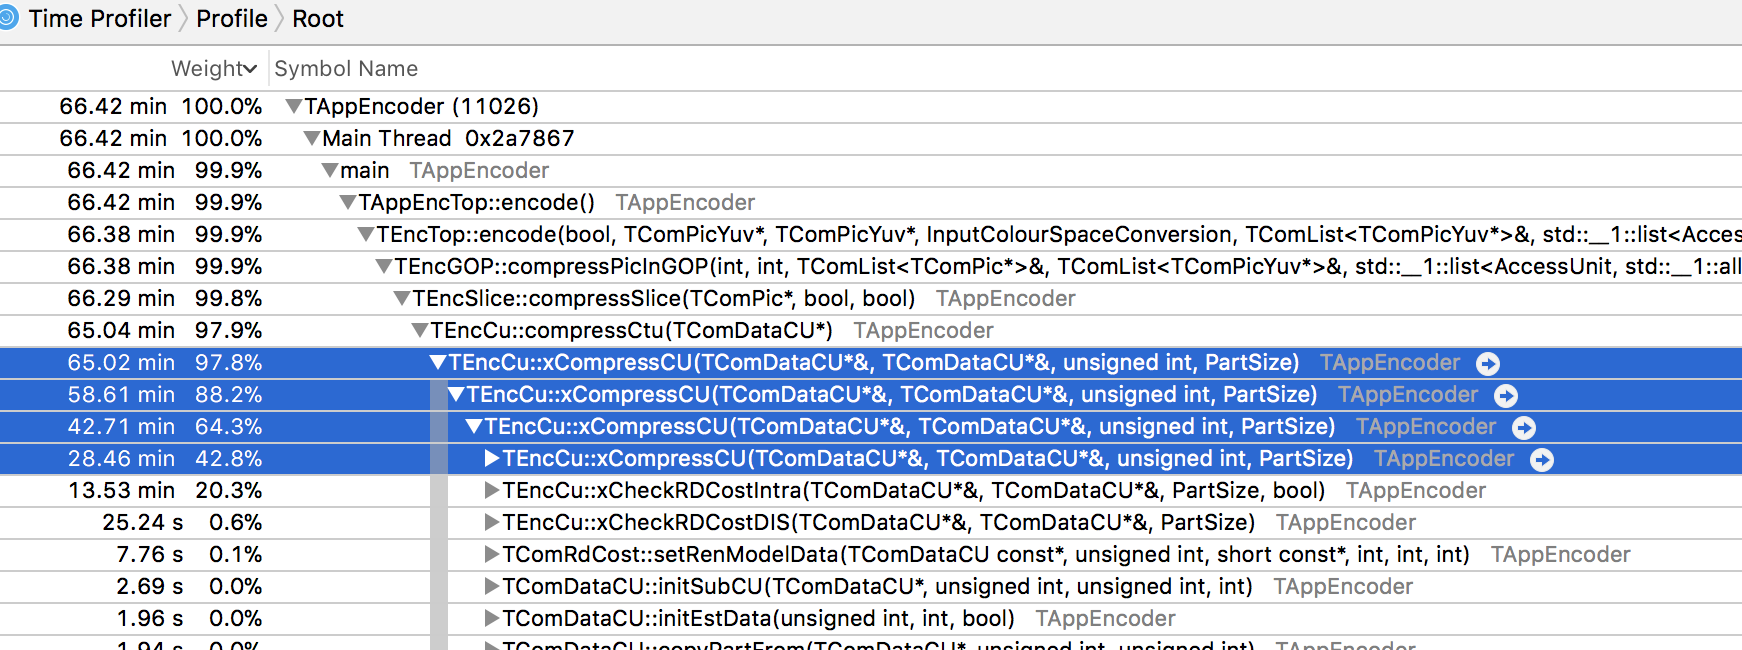
\includegraphics[width=\textwidth,height=\textheight,keepaspectratio]{Figures/major-time-spent-in-recursive-xcompresscu}
%        \decoRule
    \caption[A screen capture of the time profiling information for Newspaper sequence]
    {A screen capture of the time profiling information for Newspaper sequence.
    }\label{fig:major-time-spent-in-recursive-comresscu}
\end{figure*}
The numbers in red blocks stands for the encoding time of certain views, while
the corresponding layer Id and Picture Order Count (POD) are in the green
blocks.
A repetitive pattern of the encoding time for each view can be observed
every six numbers vertically.
A simple calculation using six numbers within the top-most
red block, \((90+69+69)/(90+69+69+14*3) \approx 0.84\), shows that
approximately 84\% of the total encoding time is busy with encoding
the depth maps.
Similarly, it is reported in~\parencite{RN111} that the coding for depth map
consumes near 86\% of total 3D-HEVC encoding time.
A trial of time profiling for 3D-HEVC encoder is performed using Instruments
which is available on macOS\@.
After encoding the Newspaper sequence for more than one hour,
Figure~\ref{fig:major-time-spent-in-recursive-comresscu} clearly shows
97.8\% time is used to compress the CUs recursively.
The first recursive xCompressCU function (denoted as XC1 thereafter) is
for CUs of size \(64\times64\), the second recursive xCompressCU
(denoted as XC2 thereafter) is targeting CUs of size \(32\times32\),
the third one (denoted as XC3 thereafter) is dedicated
to CUs of size \(16\times16\), and the last one (denoted as XC4 thereafter) is bound
to CUs of size \(8\times8\).
It is observed that the most time consuming part during the process of
compressing the depth CUs is DMM1 searching.
The DMM1 searching time percentages are summarized in
Table~\ref{tab:dmm1-searching-time-percent-summary} wherein the summary
for XC1 is omitted since DMM1 is not applicable to CUs of size 64 by 64 in
HTM-16.2.
\begin{table}[t]
    \caption{The summary of the time percentages occupied by DMM1 searching in the process for compressing CUs}
    \bigskip\label{tab:dmm1-searching-time-percent-summary}
    \centering
    \begin{tabular}{c c c}
        \toprule
        size of CU & Recursive xCompressCU Function & Time percentage of DMM1 searching process\\
        \midrule
%        Overall Display Resolution & High & Low \\
        \(32\times32\)  & XC2 & 30.0\% \\
        \(16\times16\) & XC3 & 25.6\% \\
        \(8\times8\) & XC4 & 18.8\% \\
        \bottomrule
    \end{tabular}
\end{table}[t]
The major reason leading to the time consuming property of DMM1 searching is the
View Synthesis Optimization (VSO) Method for improving quality of
synthesized views~\parencite{RN124}, wherein the Synthesized View Distortion
Change (SVDC) is computed.
The time percentages of the VSO processes in DMM1 searching are summarized in
Table~\ref{tab:vso-in-dmm1-searching-time-percent-summary}.
\begin{table}[t]
    \caption{The summary of the time percentages occupied by VSO in DMM1 searching}
    \bigskip\label{tab:vso-in-dmm1-searching-time-percent-summary}
    \centering
    \begin{tabular}{c c c}
        \toprule
        size of CU & process & Time percentage of VSO in DMM1 searching\\
        \midrule
%        Overall Display Resolution & High & Low \\
        32 by 32  & VSO in DMM1 searching from XC2 & 80.1\% \\
        16 by 16 & VSO in DMM1 searching from XC3 & 83.7\% \\
        8 by 8 & VSO in DMM1 searching from XC4 & 78.8\% \\
        \bottomrule
    \end{tabular}
\end{table}
In HTM-16.2, many wedgelet candidates are evaluated using the VSO which
has a high computational complexity.
Evaluating less wedgelet candidates will help to relieve
the burden of heavy computation required by VSO, thereby certain
time reduction can be achieved.

\textbf{Motivation for Using Deep Learning:} Deep learning such as
Multi-Layer Perceptron (MLP) is a sub field of representation learning, which
is in turn a major subset of machine learning~\parencite{RN158}.
Machine learning such as the support vector learning~\parencite{RN198}
is applied to many methods in the domain of Artificial Intelligence (AI).
%Deep Neural Network (DNN) has achieved many championships in the worldwide
%recognition contests since 2009~\parencite{RN199}.
Deep learning based on back propagation training has been found hard to proceed
in the late 1980s~\parencite{RN199}, however, starting from 2012, it kicks off the
glorious comeback.
The deep Convolutional Neural Network (CNN) has won the ImageNet
Large Scale Visual Recognition Challenge (ILSVRC)
from 2012 to 2015 with the CNN architecture of the winner going deeper
and deeper year by year.
The great achievements attract attentions from people all over the world and
make deep learning the hottest topic in our daily lives.
Inspired by the fact that supervised deep learning can learn multiple layers of
abstract representations in the visual recognition tasks, it should
be applicable to recognize the angular modes of the intra-picture
prediction in the 3D-HEVC\@.
The final DMM1 candidate selected in depth map coding
is essentially determined by the angle pattern of the depth blocks.
If we can make use of deep learning to predict the most probable angles of the
target pixel block, a vast amount of angular modes and DMM1
wedgelet candidates can be naturally skipped by which the time saving can be
achieved without decreasing the coding performance.

Motivated by the discussions above, we adopt deep learning approach with
deep convolutional neural network to accelerate the depth map coding in
3D-HEVC\@.



%%%%%%%%%%%%%%%%%%%%%%%%%%%%%%%%%%%%%%%%%%%%
% Table examples
%%%%%%%%%%%%%%%%%%%%%%%%%%%%%%%%%%%%%%%%%%%%
%\begin{table}
%    \centering
%
%    \begin{tabular}{|l||r|r|r|c|}
%        \hline
%        Name & Exam1 & Exam2 & Exam3 & Grade\\
%        \hline\hline
%        John & 19 & 28 & 33 & C\\
%        \hline
%        Jane & 49 & 35 & 60 & B\\
%        \hline
%        Jim & 76 & 38 & 59 & A\\
%        \hline
%    \end{tabular}
%
%    \caption{Math 500 Grades}
%    \label{math500grades}
%\end{table}
%
%\begin{table}
%    \label{tab:treatments}
%    \centering
%    \begin{tabular}{c r @{.} l}
%        Pi expression       &
%        \multicolumn{2}{c}{Value} \\
%        \hline
%        $\pi$               & 3&1416  \\
%        $\pi^{\pi}$         & 36&46   \\
%        $(\pi^{\pi})^{\pi}$ & 80662&7 \\
%    \end{tabular}
%    \caption{The effects of treatments X and Y on the four groups studied.}
%\end{table}
%
%\begin{table}
%    \label{tab:tabular_example1}
%    \centering
%    \begin{tabular}[t]{|r|l|}
%        \hline
%        7C0 & hexadecimal \\
%        3700 & octal \\
%        \cline{2-2} 11111000000 & binary \\
%        \hline
%        \hline
%        1984 & decimal \\
%        \hline
%    \end{tabular}
%\caption{Just an example}
%\end{table}
%
%\begin{table}
%    \label{tab:tabular_example2}
%    \centering
%    \begin{tabular}{|r|l|}
%        \hline
%        7C0 & hexadecimal \\
%        3700 & octal \\
%%        \cline{2-2}
%%        11111000000 & binary \\
%%        \hline
%%        \hline
%%        1984 & decimal \\
%        \hline
%    \end{tabular}
%\caption{Basic Usage}
%\end{table}
%
%\begin{table}
%    \label{tab:tabular_example3}
%    \centering
%    \begin{tabular}{|r|l|}
%        \hline
%        7C0 & hexadecimal \\
%        \cline{1-2}
%        3700 & octal \\
%        \cline{2-2}
%        11111000000 & binary \\
%        \cline{1-2}
%        11111000 & binary \\
%%        \hline
%%        \hline
%%        1984 & decimal \\
%        \hline
%    \end{tabular}
%\caption{horizontal lines extend over multiple columns}
%\end{table}
%
%\begin{table}
%    \label{tab:tabular_example4}
%    \centering
%    \begin{tabular}{|p{4.7cm}|}
%        \hline Welcome to Box's paragraph. We sincerely hope you'll all enjoy the show.\\
%        \hline
%    \end{tabular}
%    \caption{define a special type of column which will wrap-around the text as in a normal paragraph}
%\end{table}
%
%\begin{table}
%    \label{tab:tabular_example8}
%    \centering
%    \begin{tabular}{p{4.7cm}}
%        \hline
%        Welcome to Box's paragraph.
%        We sincerely hope you'll all enjoy the show.\\
%        \hline
%    \end{tabular}
%    \caption{define a special type of column which will wrap-around the text as in a normal paragraph}
%\end{table}
%
%\begin{table}
%    \label{tab:tabular_example5}
%    \centering
%    \begin{tabular}{@{} l @{}}
%        \hline Welcome to Box's paragraph. We sincerely hope you'll all enjoy the show.\\
%        \hline
%    \end{tabular}
%    \caption{define a special type of column which will wrap-around the text as in a normal paragraph}
%\end{table}
%
%\begin{table}
%    \label{tab:tabular_example6}
%    \centering
%    \begin{tabular}{l}
%        \hline Welcome to Box's paragraph. We sincerely hope you'll all enjoy the show.\\
%        \hline
%    \end{tabular}
%    \caption{define a special type of column which will wrap-around the text as in a normal paragraph}
%\end{table}
%
%\begin{table}
%    \label{tab:tabular_example9}
%    \centering
%    \begin{tabular}{c c} \hline \multicolumn{2}{c}{Ene} \\ \hline Me & Muh! \\ \hline \end{tabular}
%    \caption{multicolumn command}
%\end{table}
%
%\begin{table}
%    \label{tab:tabular_example10}
%    \centering
%    \begin{tabular}{c c c c c c}
%        \hline
%        sequence name &
%        BD-BR &
%        \multicolumn{4}{c}{Ene} \\
%        \cline{3-6}
%        {} & {} & Me & Muh & Me & Mu\\
%        \hline
%        Newspaper & 0.98\% & 22 & 33 & 44 & 66\\
%    \end{tabular}
%    \caption{multicolumn command}
%\end{table}




%\begin{table}
%    \label{tab:treatments}
%    \centering
%    \begin{tabular}{c r @{.} l}
%        Pi expression       &
%        \multicolumn{2}{c}{Value} \\
%        \hline
%        $\pi$               & 3&1416  \\
%        $\pi^{\pi}$         & 36&46   \\
%        $(\pi^{\pi})^{\pi}$ & 80662&7 \\
%    \end{tabular}
%    \caption{The effects of treatments X and Y on the four groups studied.}
%\end{table}
%----------------------------------------------------------------------------------------

\section{Contribution and Dissertation Outline}\label{sec:outline}
\begin{figure}
    \centering
    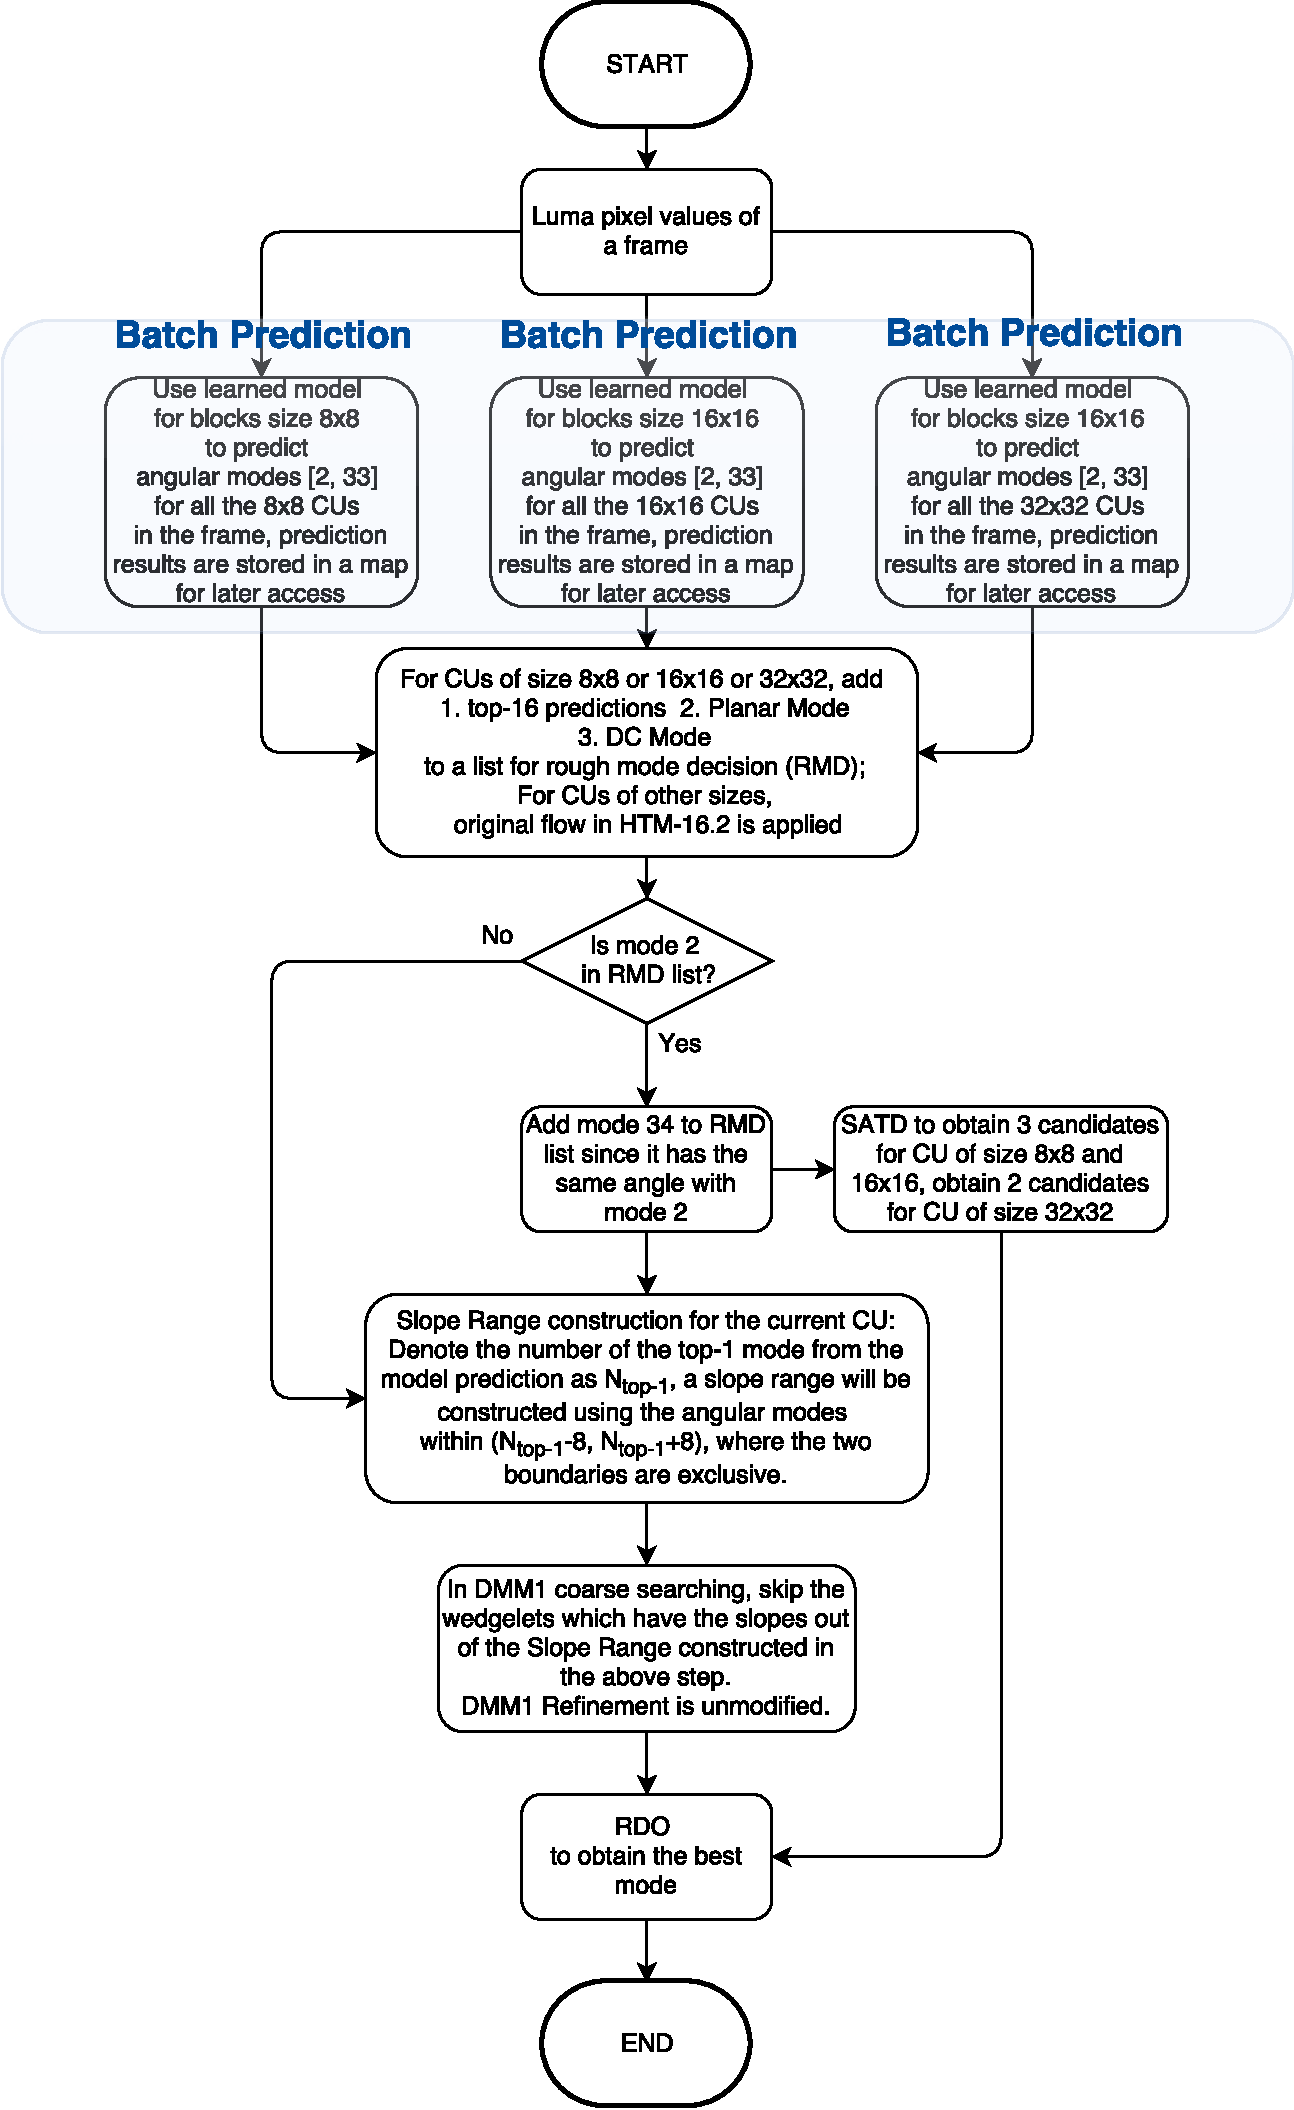
\includegraphics[width=\textwidth,height=\textheight,keepaspectratio]{Figures/proposed-fast-depth-coding-algorithm}
    \caption[Flowchart for proposed fast depth coding 
    algorithm]{Flowchart for proposed fast depth coding 
    algorithm.}\label{fig:proposed-fast-depth-coding-algorithm}
\end{figure}

We accelerate the depth map coding by leveraging the power of
deep learning.
The contributions of the dissertation are:
\begin{itemize}
  \item A deep convolutional neural network with 32 layers comprising ResNet
  units~\parencite{RN67} has been designed and trained for recognizing the
  angular directions of the blocks from intra-picture prediction in 3D-HEVC
  encoder.
  Each learned model has high top-k precision which works well on the
  tasks of recognizing intra angular patterns in 3D-HEVC\@.
  \item A way of integrating the learned model into the HTM-16.2 encoder has
  been suggested.
  By making use of Bazel~\parencite{RN200} to compile the encoder binary, the
  data level parallelism (instead of concurrency) functionality in CPU
  as well as the parallel architecture in GPU are fully utilized for
  efficient computations of matrix operations.
  \item An algorithm, illustrated in
  Figure~\ref{fig:proposed-fast-depth-coding-algorithm}
  on page~\pageref{fig:proposed-fast-depth-coding-algorithm}, for fast
  depth map coding based
  on the predictions from
  learned deep models has been proposed and implemented.
  The simulation results show that the proposed algorithm is capable of
  reducing 64.6\% time in wedgelet searching during 3D-HEVC encoding process
  while the BD performance only has a trivial decrease.
\end{itemize}
The first two contributions lay the foundation for the third one, which is the
main objective of this work: to accelerate the depth map encoding process in
3D-HEVC\@.

\textbf{Chapter~\ref{ch:chapter2}} supplies the background of video
coding history, video coding standards, and deep learning using artificial
neural network.
Prior arts in video coding and deep learning are surveyed in this chapter.

\textbf{Chapter~\ref{ch:chapter3}} describes the methodology which has been
implemented to collect the data to be used for deep learning.
The pro-processing steps for the data are provided in details along with
the reasons behind the scene.
We also visualize lots of collected data to help with the understanding of
their properties.

\textbf{Chapter~\ref{ch:chapter4}} presents the designed deep convolutional
neural network which has been applied in the deep learning process.
Both the architecture and settings
are covered in details.
The stopping criteria are shown with the training results.

\textbf{Chapter~\ref{ch:chapter5}} provides evaluation results for the
learned models.
Block resizing with different approaches are compared using the accuracy of
prediction.

\textbf{Chapter~\ref{ch:chapter6}} shows the methods been used for integrating
the learned model into the 3D-HEVC encoder.
Advantages and drawbacks of the integration are discussed.
Simulation results comparing with the original HTM-16.2 are given in this
chapter.

\textbf{Chapter~\ref{ch:chapter7}} concludes the thesis and discusses the future
work for fast depth coding using deep learning.



%\chapter{Introduction}\label{ch:chapter1} % For referencing the chapter elsewhere, use \ref{Chapter1}
%
%%----------------------------------------------------------------------------------------
%

%%----------------------------------------------------------------------------------------
%
%\section{Welcome and Thank You}\label{sec:welcome}
%Welcome to this \LaTeX{} Thesis Template, a beautiful and easy to use template for writing a thesis using the \LaTeX{} typesetting system.
%
%If you are writing a thesis (or will be in the future) and its subject is technical or mathematical (though it doesn't have to be), then creating it in \LaTeX{} is highly recommended as a way to make sure you can just get down to the essential writing without having to worry over formatting or wasting time arguing with your word processor.
%
%\LaTeX{} is easily able to~\parencite{RN93} professionally typeset documents that run to hundreds or thousands of pages long. With simple mark-up commands, it automatically sets out the table of contents, margins, page headers and footers and keeps the formatting consistent and beautiful. One of its main strengths is the way it can easily typeset mathematics, even \emph{heavy} mathematics. Even if those equations are the most horribly twisted and most difficult mathematical problems that can only be solved on a super-computer, you can at least count on \LaTeX{} to make them look stunning.
%
%%----------------------------------------------------------------------------------------
%
%\section{Welcome and Thanku}\label{sec:welome}
%Welcome to this \LaTeX{} Thesis Template, a beautiful and easy to use template for writing a thesis using the \LaTeX{} typesetting system.
%
%If you are writing a thesis (or will be in the future) and its subject is technical or mathematical (though it doesn't have to be), then creating it in \LaTeX{} is highly recommended as a way to make sure you can just get down to the essential writing without having to worry over formatting or wasting time arguing with your word processor.
%
%\LaTeX{} is easily able to professionally typeset documents that run to hundreds or thousands of pages long. With simple mark-up commands, it automatically sets out the table of contents, margins, page headers and footers and keeps the formatting consistent and beautiful. One of its main strengths is the way it can easily typeset mathematics, even \emph{heavy} mathematics. Even if those equations are the most horribly twisted and most difficult mathematical problems that can only be solved on a super-computer, you can at least count on \LaTeX{} to make them look stunning.
%
%%----------------------------------------------------------------------------------------
%
%\section{Welcome and ThYou}\label{sec:weome}
%Welcome to this \LaTeX{} Thesis Template~\parencite{Reference1}, a beautiful and easy to use template for writing a thesis using the \LaTeX{} typesetting system.
%
%If you are writing a thesis (or will be in the future) and its subject is technical or mathematical (though it doesn't have to be), then creating it in \LaTeX{} is highly recommended as a way to make sure you can just get down to the essential writing without having to worry over formatting or wasting time arguing with your word processor.
%
%\LaTeX{} is easily able to professionally typeset documents that run to hundreds or thousands of pages long. With simple mark-up commands, it automatically sets out the table of contents, margins, page headers and footers and keeps the formatting consistent and beautiful. One of its main strengths is the way it can easily typeset mathematics, even \emph{heavy} mathematics. Even if those equations are the most horribly twisted and most difficult mathematical problems that can only be solved on a super-computer, you can at least count on \LaTeX{} to make them look stunning.
%
%%----------------------------------------------------------------------------------------
%
%\section{Welcome and Thau}\label{sec:welcoe}
%Welcome to this \LaTeX{} Thesis Template, a beautiful and easy to use template for writing a thesis using the \LaTeX{} typesetting system.
%
%If you are
%\begin{table}
%
%    \label{tab:treatments}
%    \centering
%%    \begin{tabular}{l l l}
%%        \toprule
%%        \tabhead{Groups} & \tabhead{Treatment X} & \tabhead{Treatment Y} \\
%%        \midrule
%%        1 & 0.2 & 0.8\\
%%        2 & 0.17 & 0.7\\
%%        3 & 0.24 & 0.75\\
%%        4 & 0.68 & 0.3\\
%%        \bottomrule\\
%%    \end{tabular}
%    \begin{tabular}{c r @{.} l}
%        Pi expression       &
%        \multicolumn{2}{c}{Value} \\
%        \hline
%        $\pi$               & 3&1416  \\
%        $\pi^{\pi}$         & 36&46   \\
%        $(\pi^{\pi})^{\pi}$ & 80662&7 \\
%    \end{tabular}
%    \caption{The effects of treatments X and Y on the four groups studied.}
%\end{table}
%writing a thesis (or will be in the future) and its subject is technical or mathematical (though it doesn't have to be), then creating it in \LaTeX{} is highly recommended as a way to make sure you can just get down to the essential writing without having to worry over formatting or wasting time arguing with your word processor.
%
%\LaTeX{} is easily able to professionally typeset documents that run to hundreds or thousands of pages long. With simple mark-up commands, it automatically sets out the table of contents, margins, page headers and footers and keeps the formatting consistent and beautiful. One of its main strengths is the way it can easily typeset mathematics, even \emph{heavy} mathematics. Even if those equations are the most horribly twisted and most difficult mathematical problems that can only be solved on a super-computer, you can at least count on \LaTeX{} to make them look stunning.
%
%%----------------------------------------------------------------------------------------
%
%\section{Welcome and Tnk You}\label{sec:wlcome}
%Welcome to this \LaTeX{} Thesis Template, a beautiful and easy to use template for writing a thesis using the \LaTeX{} typesetting system.
%
%If you are writing a thesis.
%
%%\begin{verbatim}
%\begin{figure}
%    \centering
%    
\includegraphics{Figures/Electron}
%    %    \decoRule
%    \caption[An Electron]{An electron (artist's impression).}
%    \label{fig:Electron}
%\end{figure}
%%\end{verbatim}
%(or will be in the future) and its subject is technical or mathematical (though it doesn't have to be), then creating it in \LaTeX{} is highly recommended as a way to make sure you can just get down to the essential writing without having to worry over formatting or wasting time arguing with your word processor.
%
%\LaTeX{} is easily able to professionally typeset documents that run to hundreds or thousands of pages long. With simple mark-up commands, it automatically sets out the table of contents, margins, page headers and footers and keeps the formatting consistent and beautiful. One of its main strengths is the way it can easily typeset mathematics, even \emph{heavy} mathematics. Even if those equations are the most horribly twisted and most difficult mathematical problems that can only be solved on a super-computer, you can at least count on \LaTeX{} to make them look stunning.
%
%%----------------------------------------------------------------------------------------
